\chapter{Introduction}\label{chapter:intro}
Cluster computing applications often have high requirements to \gls{io} performance.
%
For example, many computing clusters rely on compute accelerators, such as \glspl{gpu} and \glspl{fpga}, to increase the processing speed.
%
In recent years, we have also seen a convergence of the high-performance computing, big~data, and machine~learning research fields.
%
This has led to new demands to \gls{io} performance where fast access to high-volume storage devices is becoming a requirement for high-performance computing, while low latency networking and making use of compute accelerators have become cloud computing issues~\cite{Trivedi2011,Coates2013,Taherkordi2018}.
%
If devices are distributed scarcely in the cluster, cluster machines with \gls{io} resources may become bottlenecks, for example when a workload requires heavy computation on \glspl{gpu} or fast access to storage.
%
Contrarily, over-provisioning machines with resources may lead to devices becoming underutilized if the workload's \gls{io} demands are more sporadic.
%
Heterogeneous workloads may even require widely different compositions of devices and memory resources for individual machines in the cluster.
%
Being able to share and partition devices between machines in a cluster in run-time leads to more efficient utilization, as individual machines may dynamically scale up or down \gls{io} resources based on current workload requirements.



In cloud computing environments, such dynamic scaling and resource partitioning is often handled through virtualization. 
\Gls{vm} \glspl{hypervisor} may dynamically add virtual \gls{io} devices to \gls{vm} instances on demand.
%
It is even possible to temporarily suspend computation to migrate \glspl{vm} to \gls{host} machines with more hardware resources available, should the requirements of a \gls{vm} \gls{guest} exceed the available local resources.
%
However, resource virtualization may not be viable when the raw, bare-metal \gls{io} performance is required, for example in the case of \gls{gpu}-intensive machine~learning workloads.
%
In this regard, it is possible to \lgls{passthrough}{``pass through''} physical \gls{io} devices to a \gls{vm} \gls{guest} using an \gls{iommu}.
%
The \gls{iommu} facilitates direct access to hardware from the \gls{guest} without compromising the virtualized environment.
%
Although \gls{passthrough} allows physical hardware to be used with minimal software overhead, this technique suffers from a lack of flexibility as the physical devices are tightly coupled with the hosts they are installed in.
%
Distributing VMs across hosts in the network in a way that maximizes resource utilization and adapts dynamically to varying \gls{io} requirements, without sacrificing the bare-metal performance that pass-through provides, remains a challenge.



Another challenge is the networking technology itself. 
Despite having been a research topic for decades, moving data to remote units over a network remains a costly operation that introduces large performance overheads compared to using local resources.
%
As such, many \glspl{nic} support zero-copy of application memory from one system to another through \gls{rdma}~\cite{Huang2012}.
%
\Gls{rdma} is not only used in many distributed shared-memory cluster applications, but is also frequently used for implementing \gls{io} resource \gls{disaggregation} in software.
%
For example, \glspl{nvme} may be \lgls{disaggregation}{disaggregated} and shared with remote systems with very low latency.
This is the case for \gls{nvmeof}, where \gls{rdma} is used to provide direct access and avoid going through the block-layer on the \gls{os} on the server~\cite{Guz2018}.
%
Similarly, the result of a \gls{gpu} computation may be copied out of \gls{gpu} memory and onto the network directly using \gls{rdma}, without being copied to system memory first and going through the network stack~\cite{Venkatesh2014}.
%
However, while \gls{rdma} allows data to be transferred efficiently over the network, translation between the network protocol and the local \gls{io} bus is unavoidable. 
Compared to accessing a local device, this protocol translation incurs latency overheads that are not insignificant.
%
Moreover, since \gls{rdma} requires the use of specific programming models like message-passing~\cite{Jiang2004}, \gls{disaggregation} solutions based on \gls{rdma} are usually implemented either as application-specific \gls{middleware}, or as part of the application itself.



In order to meet the latency and throughput requirements of data-driven and compute-heavy workloads in cluster computing applications,
there is a need for a solution that enables dynamic scaling and efficient sharing of resources between networked machines. 
%
This thesis contributes to this goal by ...



\section{Background and motivation}\label{sec:motivation}
\begin{figure}
	\centering
	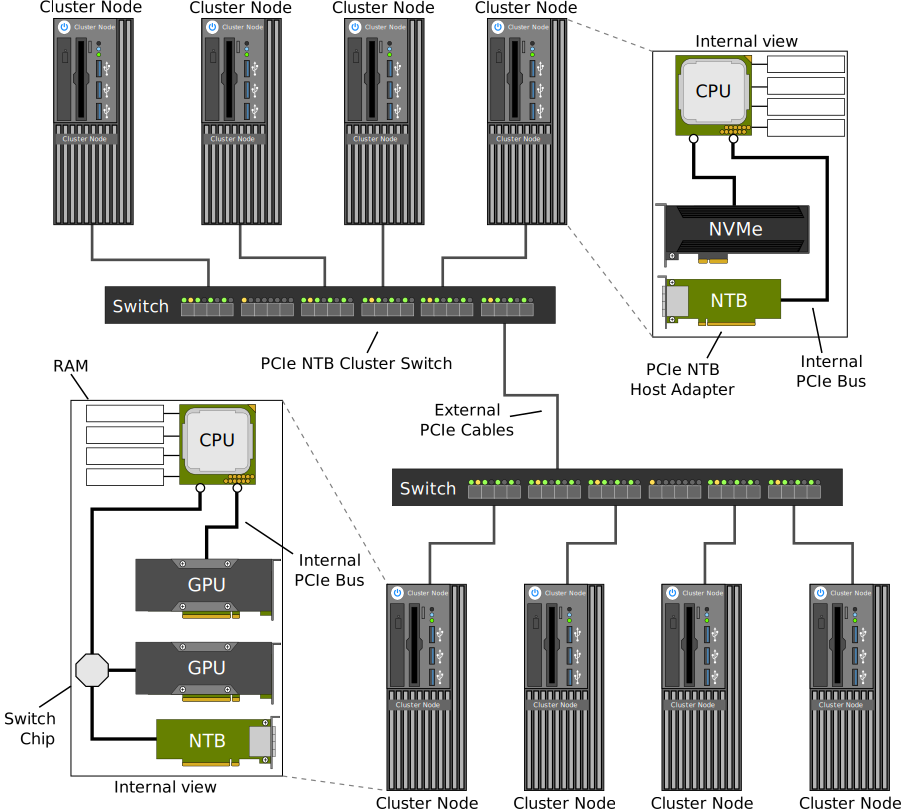
\includegraphics[width=.95\textwidth]{Cluster-Overview}
    \caption{Example of a heterogeneous \glsfmtshort{pcie}-networked cluster with external cables and adapter cards capable of \glsfmtshort{ntb}.}
  	\label{fig:cluster-example}
\end{figure}

\Gls{pcie} is the de~facto standard for connecting devices to a computer system.
%
Due to its very low latency overhead and memory addressing properties, using \gls{pcie} as a high-speed interconnection technology is a compelling alternative to traditional networking technologies~\cite{url:Meduri2011,Lim2019}.
%
However, because \gls{pcie} was originally designed for connecting devices to the \gls{cpu} on a motherboard, individual computer systems operate with different \gls{pcie} address domains.
%
Hence, extending the \gls{pcie} bus out of single computer and connecting independent systems to the same \gls{pcie} fabric requires translating memory transactions from one address domain to another.


By far, the most common way of translating addresses between different \gls{pcie} address domains is by using a special type of device called \gls{ntb}~\cite{whitepaper:PLX,whitepaper:Regula2004,Tu2018}.
%
\Glspl{ntb} can be embedded as a \gls{cpu} feature~\cite{whitepaper:Sullivan2010,url:LinuxNTB-AMD}, but are more commonly implemented in \gls{pcie} switch chips~\cite{whitepaper:PLX,pex8733}.
%
Using such \gls{ntb}-capable switch chips to implement peripheral devices, independent computer systems can interconnect with plug-in adapter cards and external cables~\cite{Ravindran2008,Lim2019,Tu2014,Tu2018}, as depicted in \cref{fig:cluster-example}.


More interesting, however, is the fact that in such \gls{pcie} networks, both \glspl{cpu} and internal \gls{pcie} devices are attached to the same, shared \gls{pcie} fabric.

The inherent memory address translation capabilities of \glspl{ntb} make it possible for a machine to map (parts of) the address space of remote systems.
%


Using \gls{pcie} networking, built with \gls{pcie} networking can allow resources to be accessed with very little performance overhead as no protocol translation between the network and the local \gls{io} bus is required.


Remote resources, such as memory and \gls{io} devices, can be mapped into a local system and accessed through the \gls{ntb}.
Similarly, a remote device capable of \gls{dma} may also use the \gls{ntb} to access local resources.

\cref{sec:tocs-intro}

%
%Remote resources, such as memory and I/O devices, can be mapped for a local system through the NTB.
%Similarly, by reverse-mapping local resources for a remote device, a device capable of DMA can access these
%resources directly. 
%
This eliminates the need to use memory on the remote node as an intermediate step when transferring data.
%
As illustrated in Figure~\ref{fig:smartio-direct-access}, 
software overhead can be avoided, since all memory address translations can be done in NTB hardware.
However, while some disaggregation approaches using NTBs have been proposed in the past~\cite{Hou2013,Tu2014}, 
%these implementations present solutions where devices are owned by a dedicated server. As distributing
%resources is generally only possible to hosts that are directly connected to the same switch as this
%server, these approaches forgo the flexibility of fully distributed cluster computing systems.
%Alternative PCIe-based solutions rely on additional virtualization functionality in the PCIe switch
%chip hardware to partition the PCIe fabric and create virtual device trees for each individual host~\cite{chung2018,microsemi2019}. 
%%
%These solutions allow devices to be directly attached a switch rather than a server. 
%%However, distributing devices is still only possible to hosts that
%%are directly connected to the same switch.
%%
%%Moreover
%However, these solutions are only able to disaggregate resources at the device level. Sharing the same
%device with multiple hosts either requires virtualization
%support in the device itself,~i.e., Single-Root I/O Virtualization~(SR-IOV), 
%or additional distribution methods, such as RDMA.





%Traditional approaches to distributed \gls{io} over network may incur additional latency overheads
%

%However, while moving data efficiently between networked nodes in a cluster has been a research challenge for decades, moving workloads and data to remote units over the network remains a costly operation that introduces large performance overheads compared to accessing local resources. 


%Consequently, \glspl{ntb} could be exploited to create a network where the inner components of all computers in the cluster,~i.e., \glspl{cpu} and \gls{pcie} devices, are connected to the same, shared \gls{pcie} fabric.
%
    %that makes it easier for nodes to scale out in order to increase overall performance in the cluster and 
    
    %seamlessly combines distributed shared-memory functionality with traditional \gls{io}, has native \gls{pcie} performance, and simultaneously makes it easier to scale out and increase overall performance in the cluster system?

%\gls{ntb}
%\gls{pcie}
%\gls{cpu}
%\gls{fpga}
%\gls{gpu}
%\gls{dma}
%\gls{os}
%\glspl{os}
%\gls{userspace}
%\gls{sriov}

%Due to its very low latency overhead and memory addressing properties, using \gls{pcie} as a high-speed interconnection technology is a compelling alternative to traditional networking technologies. 
%
%Because \gls{pcie} was originally designed as a local \gls{io} bus, connecting devices to the \gls{cpu} on a motherboard, 
%individual computer systems operate with different \gls{pcie} address domains.
%
%Interconnecting systems using \gls{pcie} require translating memory transactions from one \gls{pcie} address domain to another. 
%
%Such address translation is made possible by using \glspl{ntb}. 
%
%By using \glspl{ntb}, a computer system can map (parts of) the address space of other, remote computer systems. 

%The \gls{ntb} translate addresses between the different address domains of the independent systems.
%

%By using \glspl{ntb}, the \gls{pcie} bus of independent computers can be interconnected, creating a network fabric where the \glspl{cpu} and internal \gls{pcie} devices of all systems are directly attached.
%%
%Through such \gls{pcie} networking, scaling out and using more hardware resources than there are available in a single computer becomes possible, increasing the overall resource utilization and system performance. 
%%
%Remote resources, such as memory and devices, could be mapped into a local system and accessed through the \gls{ntb}. 
%%
%Similarly, a remote device capable of \gls{dma} could also use the \gls{ntb} to access local resources. 
%%
%However, setting up such \gls{ntb} mappings requires awareness of the address space on the remote system.
%%
%Device drivers interacting with a remote device must use addresses that corresponds with the remote device's address space.
%%
%As this greatly increases the programming complexity and require extensive modifications to existing device driver software, it is not a viable approach for enabling resource sharing among computers  as is.



\section{Problem statement}\label{sec:objectives}
Utilizing \gls{pcie} \glspl{ntb} to share resources among machines in a \gls{pcie}-networked cluster requires a 
solution for abstracting away the physical location of a resource, including the address space of the computer system it is installed in. Moreover, as it is desirable to avoid modifications to existing device drivers and application software, such a solution must also be able to present the resource to the system as if it was locally installed.
%
Hence, the goal of this thesis is to develop an infrastructure for sharing and distributing \gls{io} resources,~i.e., devices and memory, in a way that eliminates the distinction between local and remote access of a resource. The challenges of this goal are addressed under the following research question: 
\begin{restatable}{question}{researchquestion}
    % TODO: Consider making this more general for PCIe networks instead, and remove reference to NTBs
    %       From the objectives, it should be clear that NTBs are necessary anyway
    Can \glspl{ntb} be leveraged to allow the internal memory and devices of individual computers in a \gls{pcie}-networked cluster to be shared with and used by remote machines in the cluster, as if these resources were local to the remote machines?
\end{restatable}
%
In particular, this research question can be broken down into the following objectives:
%
\begin{objective}\label{obj:distributed}
    Ubiquitous sharing in the cluster should be supported, allowing any machine to contribute any of its internal \gls{pcie} devices, and allowing any machine to be able to use shared devices, even contributing and using devices at the same time.
\end{objective}
Perhaps the main motivation for our goal of building a system for \gls{io} resource sharing is to make it easier to scale out and use more resources than there are available in a single computer. 
If any standard \gls{pcie} device inside any machine could be shared with other machines, the \gls{io} resource utilization in the cluster can be greatly increased.
Additionally, by avoiding dedicated servers and allowing all computers in the cluster to participate in the sharing, contributing their own resources and using resources shared by others, we would effectively enable a distributed, peer-to-peer sharing model. This objective sets our goal apart from existing \gls{pcie}-based solutions, as these require a central server or that devices are directly attached to a \gls{pcie} switch.



\begin{objective}\label{obj:transparent}
    The fact that resources may be remote should be functionally transparent, allowing systems to use remote resources in the same way as if they were local, without requiring any modifications to device hardware, device drivers, host \gls{os}, or application software.
\end{objective}
If the solution could make remote devices behave as if they were locally installed, presenting resources to the system on a level ``underneath'' the \gls{os}, it would become possible to distribute devices to \emph{physical} hosts as well, and not only \glspl{vm}. 
In other words, remote resources should appear as if they were part of the local \gls{pcie} device tree, and application software could make use of remote devices using native interfaces the same way it would use local devices.
%
Furthermore, by avoiding application- or device-specific \gls{middleware}, and instead memory-mapping remote system and device memory directly, existing device drivers and even the host \gls{os} itself would be able to interact with remote resources natively.
Avoiding any special adaptions to software would make scaling out significantly easier than what is currently possible with existing \gls{middleware}-based solutions for distributed \gls{io}, particularly those based on \gls{rdma}.



\begin{objective}\label{obj:performance}
    The fact that resources may be remote should be transparent with regard to performance, remote resources should be used with native \gls{pcie} performance, and as close to local access as possible.
\end{objective}
Moving data to remote units over the network introduces large performance overheads compared to accessing local resources. 
In order to further blur the hard separation between ``remote'' and ``local'', remote resources should not only behave functionally as if they were locally installed in the system using them, but also have comparable performance.
To achieve this, any communication overhead and intermediate data copying in the critical path must be completely avoided, a requirement that rules out (most) traditional methods of sharing resources over a network. 
Remote resources should be accessed directly over \emph{native} \gls{pcie}, which would improve the overall \gls{io} performance in the cluster.



\begin{objective}\label{obj:dynamic}
    Shared resources should be distributed \emph{dynamically}, and direct access to device memory and system memory should be configured in run-time, also between multiple devices residing in different hosts.
\end{objective}
As stated in \cref{obj:transparent}, the solution should work for physical hosts, and not only \glspl{vm}. Therefore, it must be possible to assign and reassign resources while all machines in the cluster are running, without requiring rebooting hosts or changing settings in the \gls{bios}.
For devices, this introduces the requirement that the \gls{os} supports hot-adding devices to the system --- something most modern \gls{os} implementations do.
Not only would this would allow systems to dynamically scale up or down their \gls{io} resources based on immediate workload requirements, but devices could be more efficiently partitioned between machines in the cluster, increasing the overall resource utilization. 
Furthermore, the solution should also be able to automatically discover resource location, without requiring that the user knows anything about the underlying \gls{pcie} network topology, and dynamically set up memory-mappings between devices, \glspl{cpu}, and memory resources. An example would be enabling \gls{pcie} \gls{p2p} between two or more \gls{dma}-capable devices that are physically installed in different machines.

    
\begin{objective}\label{obj:disaggregation}
    \Gls{disaggregation} of system memory, device memory, and device \emph{functionality} should be supported, and the solution should be able to distribute component parts to different hosts, as well as provide software facilities for resources that do not support \gls{disaggregation} in hardware.
\end{objective}
Because most device drivers are written in a way that assumes exclusive control over a device, some devices implement virtualization support in hardware,~i.e., \gls{sriov}, that makes them appear to a system as having multiple \glspl{vf}. 
%
The solution should be able to \lgls{disaggregation}{disaggregate} such \gls{sriov}-capable devices, and distribute their \glspl{vf} to different machines, allowing multiple computers to use the same device simultaneously.
%
However, since not all devices implement \gls{sriov}, the solution should also provide a device driver \gls{api} that will make it possible to \lgls{disaggregation}{disaggregate} memory and device resources in software.
%
In addition to the native sharing capabilities described in \crefrange{obj:distributed}{obj:dynamic}, this \gls{api} 
would provide facilities for memory-mapping device registers as well as mapping shared memory segments for a \gls{dma}-capable device.
%
Effectively, this would bring shared-memory concepts to device driver implementations, allowing device operation and device resources to become part of the same global address space as distributed cluster applications.
%
This would allow multiple machines to simultaneously share the same, non-\gls{sriov} device, as well as making it possible to combine traditional \gls{io} with \gls{pcie} cluster capabilities such as zero-copy data transfer and multicasting.
%
Moreover, the \gls{api} should be designed so that a driver implementation does not need to consider the system-local address space of the computer system where a device is installed, thus alleviating the complexity of programming device drivers for remote devices using \glspl{ntb}.



\begin{objective}\label{obj:experiments}
    To prove real-world deployment capabilities, the solution should be tested on realistic and relevant workloads and benchmarks.
\end{objective}
To confirm that \gls{io} resources can be distributed to, and shared with, remote machines, a comprehensive performance evaluation covering all components of the implementation is needed.
As the solution should provide \emph{native} \gls{pcie} performance (\cref{obj:performance}), all parts should be thoroughly tested with latency and throughput in mind, in order to reveal any potential performance bottlenecks.
Standardized test suites should be used as far as possible, to prove that application software really can be unmodified (\cref{obj:transparent}).
%
Moreover, to demonstrate the completeness of the solution, the evaluation should also include workloads relying on different \gls{pcie} network topologies and include several types of devices, such as \glspl{nvme}, \glspl{gpu}, and \glspl{nic}.
%
Finally, a prototype device driver using the device driver \gls{api} (\cref{obj:disaggregation}) should be developed and evaluated. This driver should demonstrate that it is possible to \lgls{disaggregation}{disaggregate} a non-\gls{sriov} device in software, and shared with multiple machines simultaneously. The driver should also demonstrate how it can rely on memory \gls{disaggregation} and shared memory capabilities to implement data path optimizations.



\section{Scope and limitations}
% limitation: systems must support pcie p2p (or use switches that do)
%limitation: systems must support hot-plugging
%not disaggregated os, not general networks, not 50,000 nodes etc
% outside scope: orchestration, algorithms for sharing, fairness, etc
% scope
% both physical hosts and virtual hosts
% also shared memory applications
% distributed, unlike existing solutions, true peer-to-peer sharing
% commodity servers, multi platform amd, intel, arm

% performance, how much performance overhead in using remote devices?

% limitations
% safety, security (iommu, encryption)
% must use ntbs (dolphin ntbs), only sisci
% not a finished product (no orchistration sw [yet])
% for linux only?

\gls{sisci}
\gls{dma}

\section{Research methodology}



\section{Contributions}
The work of this thesis contributes to the topic of \gls{io} facilitation and resource sharing in distributed computing systems, and has been presented in five peer-reviewed venues: two conference workshop publications, one short-length demonstration paper, and two journal articles.
These publications are included as \crefrange{paper:nossdav}{paper:tocs} and contain the bulk of the implementation details, particularly \cref{paper:tocs} which presents the entire solution as a whole.

We have developed a system called \emph{SmartIO} for sharing resources and distributing devices in a heterogeneous, \gls{pcie}-networked cluster.
%
In particular, the main contributions of this thesis are listed as follows:
\begin{itemize}
    \item Testing and evaluation of the \emph{Device~Lending} mechanism for \textbf{distributing \gls{pcie} devices to remote systems} (see \cref{paper:nossdav} and \cref{paper:mmsys}). Using Device~Lending, any standard \gls{pcie} device, such as \glspl{nvme}, \glspl{gpu}, \glspl{nic}, and \glspl{fpga}, may be assigned to a remote system. The device appear to the remote system as if it has been dynamically hot-added to the system, allowing existing device drivers to use the device without requiring any modifications to software.

    \item Implementation of a \textbf{new mechanism for distributing devices to \glspl{vm}} running on any host machine in the cluster (see \cref{paper:srmpds} and \cref{paper:cc}). We have developed an extension to \gls{kvm} based on the \emph{\gls{mdev}} interface, enabling direct access to remote physical hardware devices for \gls{vm} guests and setting up memory mappings for the devices. This \gls{mdev} implementation includes a method for dynamically discovering guest-physical memory layout. Using this \gls{mdev} extension, local and remote devices can be \lgls{passthrough}{``passed through''} to \glspl{vm} and used with bare-metal performance.
	
    \item Improvement of the Device~Lending and \gls{kvm}/\gls{mdev} mechanisms by implementing \textbf{support for multiple devices} and \textbf{supporting devices in different physical machines} (see \cref{paper:srmpds} and \cref{paper:cc}). A method for resolving device memory addresses and setting up memory mappings, in a way that is transparent to both the devices and the device drivers, is implemented. This enables direct data transfers between multiple devices without violating the principle of making devices appear local to the system(s) using them.

    \item Extension of the \gls{sisci} shared-memory \gls{api} with new, \textbf{device-oriented programming semantics} for writing device drivers as shared-memory applications (see \cref{paper:tocs}).
    %
	This \gls{api} extension makes it possible to \lgls{disaggregation}{disaggregate} devices and device memory in software, similarly to \gls{rdma} \gls{disaggregation} solutions.
	Unlike \gls{rdma} solutions, however, remote resources can be memory-mapped directly into the virtual address space of a software process.
	%
	Through our \gls{api} extension, device driver implementations may take full advantage of \gls{pcie} shared memory capabilities, such as remote memory access and multicasting, without requiring awareness of the underlying \gls{pcie} topology and the different address domains of remote systems.
	%
	This makes it easier to optimize data flow through the \gls{pcie} network, as software no longer needs to be written with accessing remote resources in mind, but can be implemented as if resources are local.

    \item Development of a \textbf{new prototype \gls{nvme} device driver} using our device-oriented \gls{api} extension (see \cref{paper:tocs}).\footnote{The prototype \gls{nvme} device driver is open source and can be found at \mbox{\url{https://github.com/enfiskutensykkel/ssd-gpu-dma}}}
    Although the Device~Lending mechanism and \gls{mdev} extension makes it possible to use existing device drivers, most device drivers are written in a way that assumes exclusive control over the device. Therefore, a distributed device (function) may only be used by a single user at the time.
    To demonstrate software-enabled \gls{disaggregation}, we have implemented a \emph{distributed} \gls{nvme} driver. As a proof of concept, we show a single NVMe device can be shared and operated by multiple cluster machines simultaneously, without requiring \gls{sriov}.
	This driver also demonstrates how multiple sharing aspects of SmartIO may be combined, 
	by \lgls{disaggregation}{disaggregating} remote GPU memory and enabling memory access optimizations.

    \item A \textbf{comprehensive performance evaluation} covering all parts of SmartIO and the implementation of performance optimizations (see \cref{paper:mmsys}, \cref{paper:cc}, and \cref{paper:tocs}). With the goal of not incurring any performance overhead beyond that of native \gls{pcie}, the performance of using remote resources with SmartIO is comparable to that of local access (in terms of latency and throughput).
        To prove that SmartIO is a viable and efficient solution for \gls{io} resource sharing also for realistic scenarios, two different image classification workloads relying on multiple \glspl{gpu} and \gls{nvme} storage have also been tested.
	
\end{itemize}
%
Finally, it should be noted that the research of this thesis has had impact on real systems, as several components of SmartIO have already been incorporated into the product line of Dolphin Interconnect Solutions, and others are currently being adapted for real-world deployment.\footnote{{\url{https://www.dolphinics.com/solutions/pcie_smart_io.html}}}


\section{Outline}
This thesis describes the SmartIO system for efficient sharing of resources between \gls{pcie}-networked computers.
%
The rest of this thesis is organized as follows:
\begin{description}
    \item[\cref{chapter:smartio}]
        presents the overall ideas and challenges for SmartIO. 
        We give a high-level overview of the implementation and 
        also related work

    \item[\cref{chapter:conclusion}]

    \item[\cref{paper:nossdav}]

    \item[\cref{paper:mmsys}]

    \item[\cref{paper:srmpds}]

    \item[\cref{paper:cc}]

    \item[\cref{paper:tocs}]
\end{description}

